\documentclass[a4paper]{article}

\usepackage[latin1]{inputenc} \usepackage{microtype}
\usepackage{fancyhdr} \usepackage{amsmath} %\text in math
\usepackage{hyperref}
\usepackage{graphicx}

\newcommand*{\plogo}{\fbox{Ullern VGS - Teknologi \& Forskningsl�re}}
% Generic publisher logo

%----------------------------------------------------------------------------------------
%	TITLE PAGE
%----------------------------------------------------------------------------------------

\newcommand*{\titleGM}{\begingroup % Create the command for including the title page in the document
\thispagestyle{plain}%No page style from fancthdr
\hbox{ % Horizontal box
\hspace*{0.2\textwidth} % Whitespace to the left of the title page
\rule{1pt}{\textheight} % Vertical line
\hspace*{0.05\textwidth} % Whitespace between the vertical line and title page text
\parbox[b]{0.75\textwidth}{ % Paragraph box which restricts text to  less than the width of the page

{\noindent\Huge\bfseries Autonome biler \\ \hspace*{5pt}\LARGE -Teknologi
  \& Forskningsl�re}\\[2\baselineskip] % Title
{\large
\textit{Utkast}}\\[4\baselineskip] % Tagline or further description
{\Large \textsc{Thorvald Molthe Ballestad}} %Author name

\vspace{0.5\textheight} % Whitespace between the title block and the publisher
{\noindent \plogo}\\[\baselineskip] % Publisher and logo
}}
\endgroup}

\pagestyle{fancy} \rhead{\leftmark}
%\rfoot{\plogo}
\cfoot{\thepage}

\fancypagestyle{plain}{ \fancyhf{} \renewcommand{\headrulewidth}{0pt}
}

\renewcommand{\abstractname}{Abstrakt}

\begin{document}

\titleGM % This command includes the title page

\tableofcontents
\newpage

\begin{abstract}
Mennesker har i alle tider utviklet hjelpemiddler for � gj�re hverdagen lettere, dette kan beskrives som automatisering. Intill helt nylig har man kun hatt fysisk automatisering, men n� kommer kognitiv automatisering for fult. Jeg vil se p� denne teknologien, hovedsakelig autonome biler, og p� hvordan dette vil p�virke det samfunnet vi lever i.
\end{abstract}

\section{Teknologien}
Autonome biler er gjort mulig hovedsakelig p� grunn av en enorm utvikling innenfor software og sensor-teknologi.
\subsection{Software \& sensor}
Autonome biler bruker flere avanserte sensorer for � kartlegge omgivelsene sine. Ulike prosjekter og tilnerminger bruker ulik teknologi, men de fleste baserer seg hovedsakelig p� 4 hovedsystemer: gps, akselerasjon \& gyroskop, kamera og radar.
\subsection{Aktiv kontroller}
http://www.templetons.com/brad/robocars/
\subsection{Mekanisk teknologi}

\section{Teknologi utkast 2}
Siden dette er en teknologi i en veldig tidlig fase, med potensiellt stor profitt, forteller akt�rene lite spesiffikt om teknologien de bruker. Jeg vil se p� det grunnleggende innenfor de viktigste sensorene og teknikkene.
\subsection{Kontroller}
Kontroll teori er viktig for autonome biler. Kontroll teori er l�ren om dynamiske systemer og hvordan man kan endre oppf�reselen til systemer basert p� responser fra systemet\cite{wiki:control-theory}.
\begin{figure}[ht]
\begin{center}
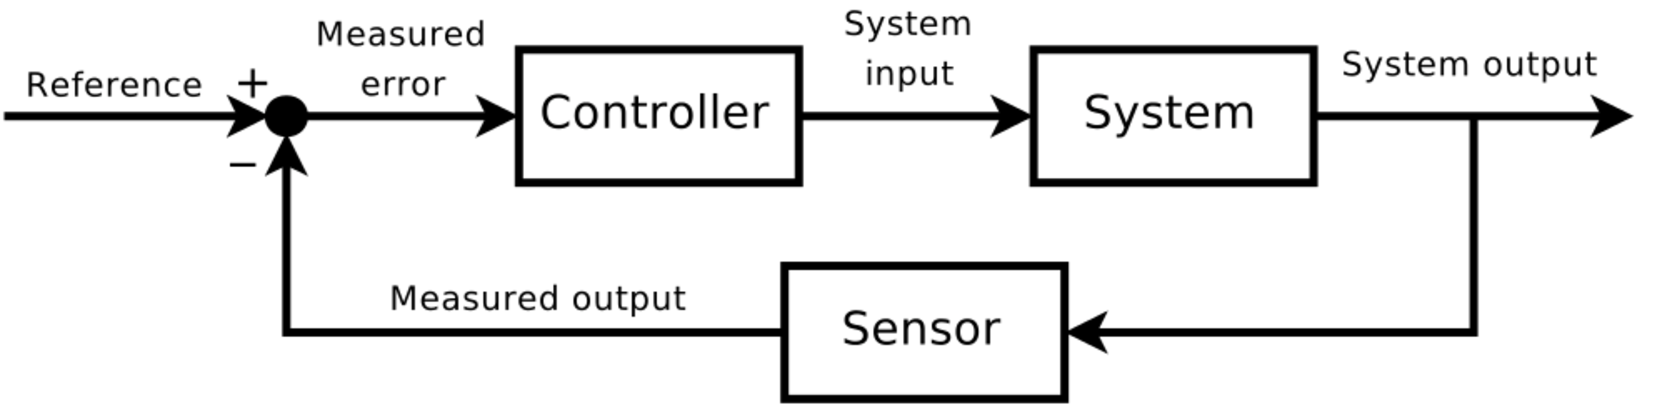
\includegraphics[width=0.75\textwidth]{controller2}
\caption{"Feedback loop with descriptions" by Myself - Own work. Licensed under GNU Free Documentation License via Wikimedia Commons - \url{https://commons.wikimedia.org/wiki/File:Feedback_loop_with_descriptions.svg\#mediaviewer/File:Feedback_loop_with_descriptions.svg}}
\end{center}
\end{figure}

Det grunnleggende konseptet med en kontroll algoritme er � g� utifra en �nsket verdi, og s� justere inputen til systemet for � oppn� dette. Et eksempel p� en slik situasjon er n�r man kj�rerer bil og �nsker � holde en viss fart. Da er farten referansepunktet, eller den �nskede verdien, og den faktiske verdien vil v�re det som vises p� speedometeret, som er \emph{sensoren}. S� lenge veien er flat og har lik friksjon vil inputen v�re konstant; den m�lte feilen er 0, \emph{referansen-feilen}. Hvis bilen kommer til en bakke derimot, m� man enten �ke eller minke inputen for � holde den �nskede farten.

Kontrolleren er en algoritme som skal minimere feilen s� fort som mulig, innenfor de premissene som er gitt av systemet; i noen systemer vil det for eksempel v�re viktigst � minimere den maksimale feilverdien, p� bekostning av at det tar lengre tid � rette opp i feilen, der andre systemer kan godta store feil i korte perioder.
\begin{figure}[ht]
\begin{center}
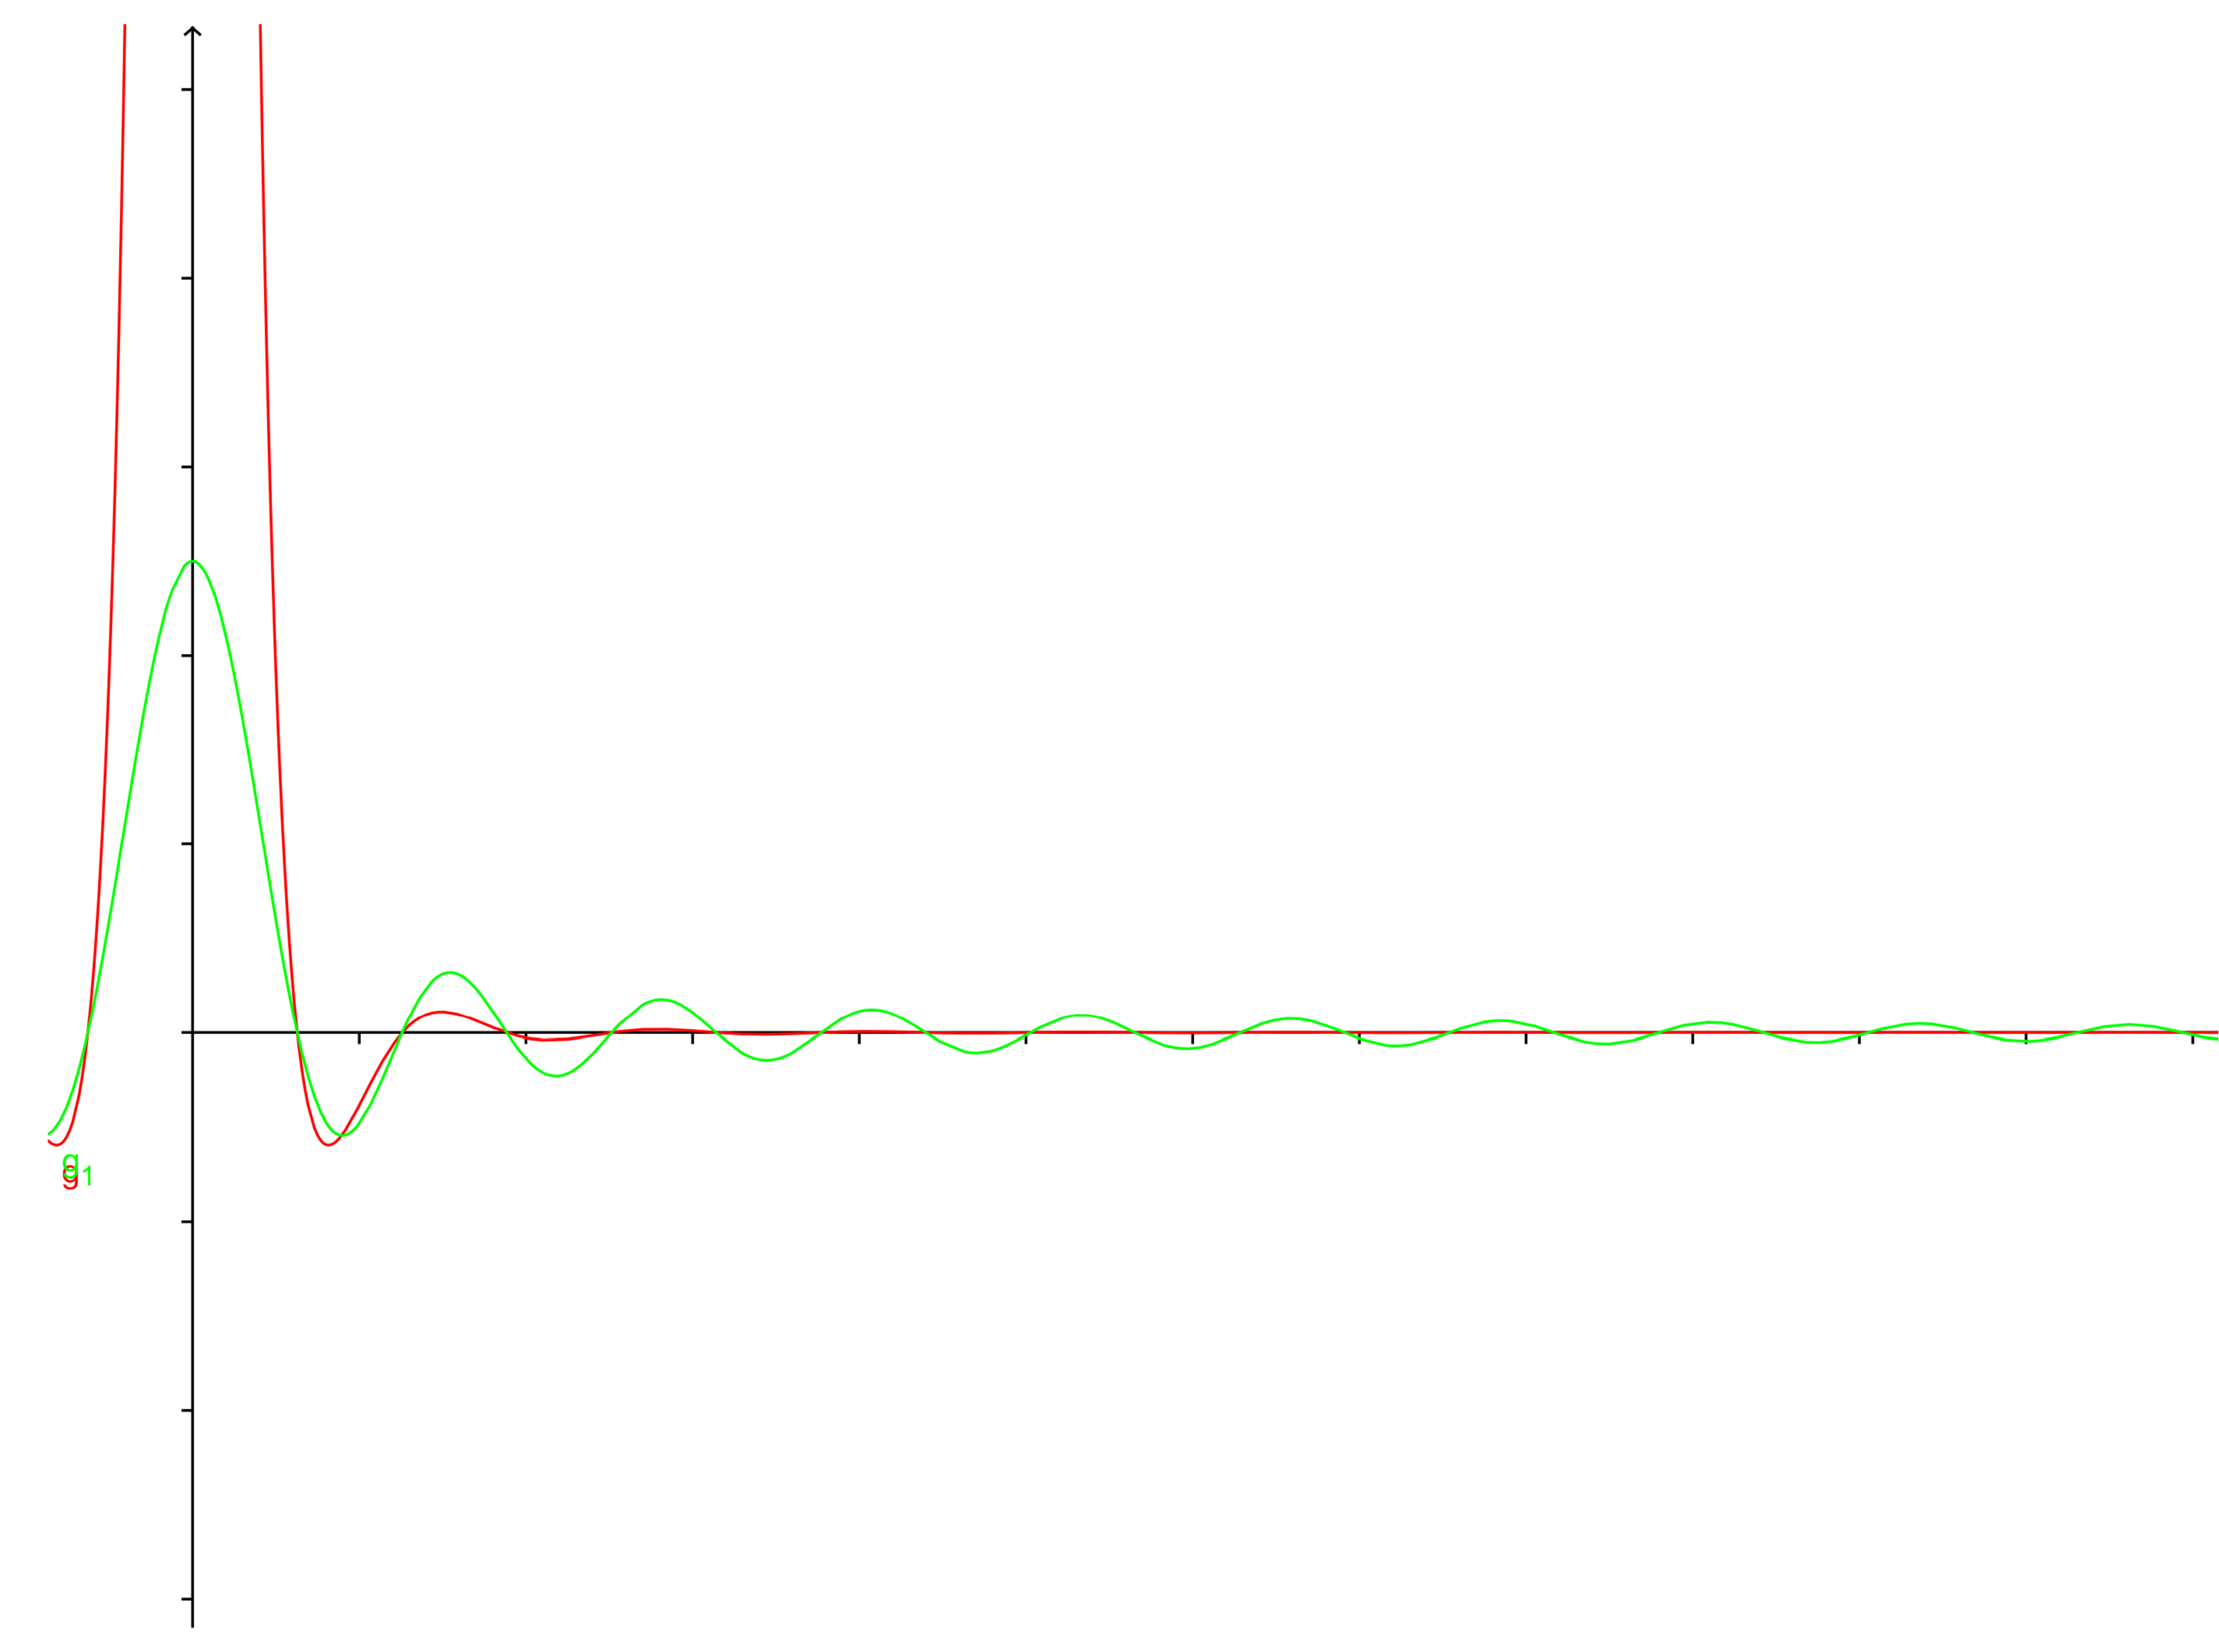
\includegraphics[width=0.75\textwidth]{pid}
\end{center}
\end{figure}
\subsection{LIDAR og RADAR}
\subsection{Grafisk gjennkjennelses-programvare}

\section{Kj�reegenskaper}

\section{�konomi \& samfunn}

\section{Utfordringer \& problemer}
\begin{itemize}
\item Etiske problemer
\begin{itemize}
\item http://www.theatlantic.com/technology/archive/2013/10/the-ethics-of-autonomous-cars/280360/
\item http://www.forbes.com/sites/timworstall/2014/06/18/when-should-your-driverless-car-from-google-be-allowed-to-kill-you/
\item The trolley problem
http://en.wikipedia.org/wiki/Trolley\_problem
\end{itemize}
\item Juridiske problemer
\end{itemize}

\begin{itemize}
\item www.youtube.com/watch?v=1BylX2XwwAM
\end{itemize}


\begin{thebibliography}{9}


\bibitem{wiki:control-theory} Control theory. Wikipedia.org \url{https://en.wikipedia.org/wiki/Control_theory}
\end{thebibliography}
\end{document}
